%
%	Diploma thesis template 2005
%
%       author: lukas.silberbauer(at)gmx.at
%       based upon  "Diplomarbeit mit LaTeX" by Tobias Erbsland
%
%       published under the terms of
%
%  ----------------------------------------------------------------------------
%  "THE BEER-WARE LICENSE":
%  <lukas.silberbauer(at)gmx.at> wrote this file. As long as you retain this 
%	notice you can do whatever you want with this stuff. If we meet some day, 
%	and you thinkthis stuff is worth it, you can buy me a beer in return. 
%  ----------------------------------------------------------------------------
%

% %	Diploma thesis template 2005
%
%       author: lukas.silberbauer(at)gmx.at
%       based upon  "Diplomarbeit mit LaTeX" by Tobias Erbsland
%
%       published under the terms of
%
%  ----------------------------------------------------------------------------
%  "THE BEER-WARE LICENSE":
%  <lukas.silberbauer(at)gmx.at> wrote this file. As long as you retain this 
%	notice you can do whatever you want with this stuff. If we meet some day, 
%	and you think this stuff is worth it, you can buy me a beer in return. 
%  ----------------------------------------------------------------------------

%
% header.tex
%
\documentclass[%
	pdftex,%              PDFTex verwenden
	a4paper,%             A4 Papier
	oneside,%             Einseitig
	bibtotocnumbered,%    Literaturverzeichnis nummeriert einf�gen
	idxtotoc,%            Index ins Verzeichnis einf�gen
	halfparskip,%         Europ�ischer Satz mit abstand zwischen Abs�tzen
	chapterprefix,%       Kapitel anschreiben als Kapitel
	%headsepline,%         Linie nach Kopfzeile
	%footsepline,%         Linie vor Fusszeile
	12pt%                 Gr��ere Schrift, besser lesbar am bildschrim
]{scrbook}


%
% Paket f�r die Indexerstellung.
%
\usepackage{makeidx}

%
% Paket f�r �bersetzungen ins Deutsche
%
\usepackage[german, english]{babel}

%
% Pakete um Latin1 Zeichnens�tze verwenden zu k�nnen und die dazu
%  passenden Schriften.
%
\usepackage[latin1]{inputenc}
\usepackage[T1]{fontenc}

%
% Paket zum Erweitern der Tabelleneigenschaften
%
\usepackage{array}

%
% Paket um Grafiken einbetten zu k�nnen
%
\usepackage{graphicx}

%
% Spezielle Schrift verwenden.
%
\renewcommand{\encodingdefault}{T1}
%\renewcommand{\familydefault}{goudysans}
\renewcommand{\familydefault}{\sfdefault}


%
% Zeilenabstand einstellen
%
\usepackage{setspace}
\onehalfspacing
%\doublespacing

%\setlength{\baselineskip}{24pt}
%\renewcommand{\baselinestretch}{1.5} 

%
% define variables
%
\def\maintitle#1{\gdef\maintitle{#1}}
\def\subtitle#1{\gdef\subtitle{#1}}

%
% Zeilenumbruch bei Bildbeschreibungen.
%
\setcapindent{1em}

%
% kopf und fusszeilen
%
\pagestyle{headings}

%
% mathematische symbole aus dem AMS Paket.
%
\usepackage{amsmath}
\usepackage{amssymb}

%
% Type 1 Fonts f�r bessere darstellung in PDF verwenden.
%
\usepackage{mathptmx}           % Times + passende Mathefonts
\usepackage[scaled=.75]{helvet} % skalierte Helvetica als \sfdefault
\usepackage{courier}            % Courier als \ttdefault

%
% Paket um Textteile drehen zu k�nnen
%
\usepackage{rotating}

\usepackage{verbatim,framed}
\usepackage{moreverb}

%
% F�r Acronyme
%
\usepackage{acronym}

%
% Package f�r Farben im PDF
%
%\usepackage{color}
\usepackage[dvipsnames]{color}
\usepackage[dvipsnames,svgnames]{pstricks}

%
% Paket f�r Links innerhalb des PDF Dokuments
%
\definecolor{LinkColor}{rgb}{0,0,0.5}

\usepackage[%
pdfauthor={Paul B\"{u}tow},
bookmarks=true, % PDF bookmarks allowed. NB! The level depth of bookmarks is the same as in the TOC.
unicode=true, % PDF bookmarks in Unicode.
bookmarksnumbered=true, % Section numbers in PDF bookmarks.
bookmarksopenlevel=1, % The open level in PDF bookmarks.
hyperindex=true, % Hyperlinked index.
colorlinks=true, % Links are marked as coloured text, not coloured box.
linkcolor=linkc, % The colour for in-document links (e.g. in the table of contents).
citecolor = citec, % The colour for bibliographic citations.
urlcolor=urlc, % The colour for hyperlinks to the Net.
pdfpagelayout=OneColumn % Continuous page scrolling.
]{hyperref}
\hypersetup{colorlinks=true,%
	linkcolor=LinkColor,%
	citecolor=LinkColor,%
	filecolor=LinkColor,%
	menucolor=LinkColor,%
	pagecolor=LinkColor,%
	urlcolor=LinkColor}

%
% Paket um Listings sauber zu formatieren.
%
\usepackage[savemem]{listings}
\lstloadlanguages{TeX}

%
% ---------------------------------------------------------------------------
% Listing Definationen f�r PHP Code
%
\definecolor{lbcolor}{rgb}{0.85,0.85,0.85}
\lstset{language=[LaTeX]TeX,
	numbers=left,
	stepnumber=1,
	numbersep=5pt,
	numberstyle=\tiny,
	breaklines=true,
	breakautoindent=true,
	postbreak=\space,
	tabsize=2,
	basicstyle=\ttfamily\footnotesize,
	showspaces=false,
	showstringspaces=false,
	extendedchars=true,
	backgroundcolor=\color{lbcolor}}

% ---------------------------------------------------------------------------
% Neue Umgebungen
% ---------------------------------------------------------------------------

\newenvironment{ListChanges}%
	{\begin{list}{$\diamondsuit$}{}}%
	{\end{list}}

\newenvironment{code}%
{%
\definecolor{shadecolor}{named}{LightYellow}%
\topsep=0ex\relax
\framed
\small
\verbatim
}%
{%
\endverbatim
\endframed
}%

%
% Index erzeucgen
%
\makeindex

%
% EOF
%


%%%%%%%%%%%%%%%%%%%%%%%%%%%%%%%%%%%%%%%%%%%%%%%%%%%%%%%%%%%%%%%%%%%%%%
%
% define variables used on titlepage
%
%%%%%%%%%%%%%%%%%%%%%%%%%%%%%%%%%%%%%%%%%%%%%%%%%%%%%%%%%%%%%%%%%%%%%%

\maintitle {Objektorientierte Entwicklung eines GUI-basierten Tools f\"{u}r die Simulation ereignisbasierter verteilter Systeme}
\subtitle { ~ }

%%%%%%%%%%%%%%%%%%%%%%%%%%%%%%%%%%%%%%%%%%%%%%%%%%%%%%%%%%%%%%%%%%%%%%
%
% setup document structure
%
%%%%%%%%%%%%%%%%%%%%%%%%%%%%%%%%%%%%%%%%%%%%%%%%%%%%%%%%%%%%%%%%%%%%%%

\begin{document}
%	Diploma thesis template 2005
%       author: lukas.silberbauer(at)gmx.at
%       based upon  "Diplomarbeit mit LaTeX" by Tobias Erbsland
%       published under the terms of
%  ----------------------------------------------------------------------------
%  "THE BEER-WARE LICENSE":
%  <lukas.silberbauer(at)gmx.at> wrote this file. As long as you retain this notice 
%  you can do whatever you want with this stuff. If we meet some day, and you think
%  this stuff is worth it, you can buy me a beer in return. 
%  ----------------------------------------------------------------------------

\selectlanguage{german}
\begin{titlepage} % enlarge page
	\pagestyle{empty}
	\setlength{\topmargin}{0pt}
	\setlength{\headheight}{0pt}
	\setlength{\headsep}{0pt}
	\setlength{\footskip}{0pt}	
	\begin{center}
		\begin{figure}[ht]
			\centering
				
\includegraphics{images/fhac_logo.png}
			\label{fig:tulogo}
		\end{figure}
	
		\vspace*{1cm}
						
		{\Huge\bf DIPLOMARBEIT \\[1cm]}
		{\Large\bf {\maintitle} \\}
		
		{~\\Durchgef�hrt an der}

		{\large Fachhochschule Aachen\\}
		{\large Fachbereich Elektrotechnik und Informationstechnik}

		{Eupener Str. 70\\}
		{D-52066 Aachen\\~\\}
		
		{mit Erstpr\"{u}fer und Betreuer }
		{\large Prof. Dr.-Ing. Martin O�mann}

		{und Zweitpr\"{u}fer}
		{\large Prof. Dr. rer. nat. Heinrich Fassbender}
		
		{durch\\}
		{\large\bfseries Paul C. B\"{u}tow\\[0.3cm] }
		{\large Matr.Nr.: 266617\\}
		{Matthiashofstr. 15\\}
		{D-52064 Aachen\\}
	\end{center}
	
	\vspace*{0.5cm}
	
	\begin{flushleft}
	{Aachen, den \today \\}
	\end{flushleft}

\end{titlepage}
%\selectlanguage{german}

\vspace*{2cm}
\textbf{\LARGE Danksagungen}
\vspace*{1.5cm}

Ohne die Hilfe folgender Personen w\"{a}re die Anfertigung dieser Diplomarbeit in diesem Ma�e nicht m\"{o}glich gewesen. Daher m\"{o}chte ich mich bedanken bei:

\begin{itemize}
	\item Prof. O�mann als 1. Pr\"{u}fer sowie Prof. Fassbender als 2. Pr\"{u}fer
	\item Andre Herbst
	\item Carrie Callahan 
	\item Florian B\"{u}tow
	\item J\"{o}rn B\"{u}tow
	\item Leslie B\"{u}tow
\end{itemize}

Auch vielen Dank an die Open Source Gemeinde, denn diese Diplomarbeit wurde ausschlie�lich mit Hilfe von Open Source Software angefertigt

\tableofcontents

\listoffigures

\listoftables


\chapter{Einleitung}

\section{Motivation}

In der Literatur findet man viele verschiedene Definitionen eines verteilten Systems. Vieler dieser Definitionen unterschieden sich untereinander, so dass es schwer f�llt eine Definition zu finden, die als Alleinige als die Richtige gilt. Andrew Tanenbaum und Marten van Steen haben f�r die Beschreibung eins verteilten Systems die Folgende lockere Charakterisierung formuliert:

\cite{Tanenbaum} \textit{``Ein verteiltes System ist eine Menge voneinander unabh�ngiger Computer, die dem Anwender wie ein einzelnes, koh�rentes System erscheinen''}

Der Anwender muss sich nur mit dem lokalen vor ihm befindenden Computer auseinandersetzen, w�hrend die Software des lokalen Computers die reibungslose Kommunikation mit den anderen beteiligten Computern des verteilten Systems sicherstellt.

Diese Diplomarbeit soll den Gebrauchern die Betrachtung von verteilten Systemen aus einer anderen Perspektive erleichtern. Es soll nicht die Sichtweise eines Endbenutzers eingenommen werden, sondern es sollen die Funktionsweisen von Protokollen und deren Prozesse in verteilten Systemen begreifbar gemacht werden. Es sollen relevante Ereignisse eines verteilten Systems transparent dargestellt werden k�nnen. 

Um dieses Ziel zu erreichen soll ein Simulator entwickelt werden. Der Simulator soll insbesondere f�r Lehr- und Lernzwecke an der Fachhochschule Aachen entwickelt werden. Beispielsweise sollen Protokolle aus den verteilten Systemen mit ihren wichtigsten Einflussfaktoren simuliert werden k�nnen. Der Simulator soll zu verstehen helfen wie die gegebenen Protokolle funktionieren und es soll viel Spielraum f�r eigene Experimente zur Verf�gung stehen. Der Simulator soll nicht auf eine feste Anzahl von Protokollen beschr�nkt sein. Es muss daher dem Gebraucher erm�glicht werden, eigene Protokolle zu entwerfen.

\section{Grundlagen}

F�r das Grundverst�ndnis werden im Folgenden einige Grundlagen erl�utert. Eine Vertiefung findet erst in den sp�teren Kapiteln statt.

\subsubsection{Client/Server Modell}

\begin{figure}[htbp]
	\centering
	\fbox{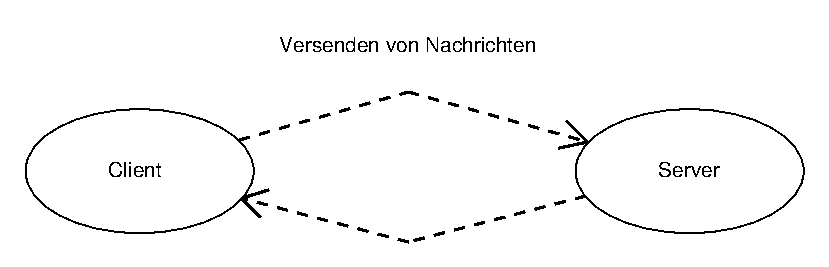
\includegraphics{images/client-server}}
	\caption{Client/Server Modell}
	\label{fig:ClientServer}
\end{figure}

Der Simulator basiert auf dem Client/Server Prinzip. Jeder Simulation besteht in der Regel aus einen teilnehmenden Client und einen Server, die miteinander �ber Nachrichten kommunizieren (Abbildung \ref{fig:ClientServer}). Bei komplexen Simulationen k�nnen auch mehrere Clients und/oder Server mitwirken. 

\subsubsection{Prozesse und deren Rollen}

Ein verteiltes System wird anhand von Prozessen simuliert. Jeder Prozess nimmt hierbei eine oder mehrere Rollen ein. Beispielsweise kann ein Prozess die Rolle eines Clients einnehmen und ein weiterer Prozess die Rolle eines Servers. Ein Prozess kann auch Client und Server gleichzeitig sein. Es besteht auch die M�glichkeit, dass ein Prozess die Rollen mehrerer Server und Clients gleichzeitig einnimmt. Ob das sinnvoll ist h�ngt vom simulierten Szenario ab. Um einen Prozess zu kennzeichnen besitzt jeder Prozess eine \textbf{eindeutige} Prozess-Identifikationsnummer (PID). 

\subsubsection{Nachrichten}

In einem verteiltem System m�ssen Nachrichten verschickt werden k�nnen. Eine Nachricht kann von einem Client- oder Serverprozess verschickt werden und kann beliebig viele Empf�nger haben. Der Inhalt einer Nachricht h�ngt vom verwendeten Protokoll ab. Was unter einem Protokoll zu verstehen ist, wird sp�ter behandelt. Um eine Nachricht zu kennzeichnen besitzt jede Nachricht eine \textbf{eindeutige} Nachrichten-Identifikationsnummer (NID).

\subsubsection{Lokale und globale Uhren}

In einer Simulation gibt es \textbf{genau eine} globale Uhr. Sie stellt die aktuelle und \textbf{immer korrekte} Zeit dar. Eine globale Uhr geht nie falsch.

\begin{figure}[htbp]
	\centering
	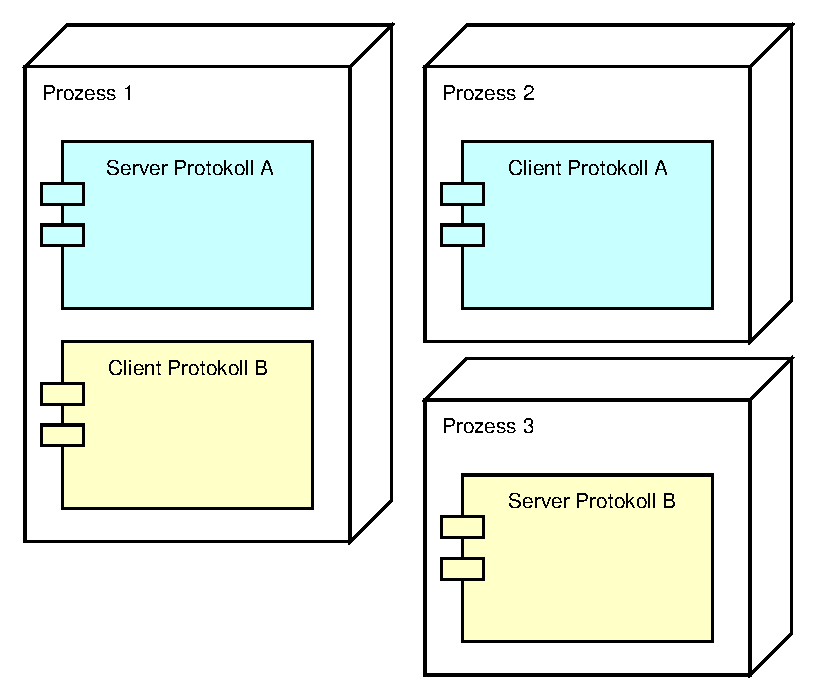
\includegraphics{images/client-server-protokolle}
	\caption{Client/Server Protokolle}
	\label{fig:ClientServerProtokolle}
\end{figure}

Zudem besitzt jeder beteiligter Prozess eine eigene lokale Uhr. Sie stellt die aktuelle Zeit des jeweiligen Prozesses dar. Im Gegensatz zu der globalen Uhr k�nnen lokale Uhren eine falsche Zeit anzeigen. Wenn die Prozesszeit nicht global-korrekt ist (nicht der globalen Zeit gleicht beziehungsweise eine falsche Zeit anzeigt), dann wurde sie entweder im Laufe einer Simulation neu gestellt, oder sie geht wegen einer Uhrabweichung falsch. Die Uhrabweichung gibt an, um welchen Faktor die Uhr falsch geht. Hierauf wird sp�ter genauer eingegangen. 

Neben den normalen Uhren sind auch die Vektor-Zeitstempel sowie die logischen Uhren von Lamport von Interesse. Jeder Prozess besitzt zus�tzlich einen Vektor-Zeitstempel f�r seine Vektorzeit, sowie einen Lamportzeitstempel f�r seine Lamportzeit. F�r die Vektor- und Lamportzeiten gibt es hier, im Gegensatz zu der normalen Zeit, keine globalen �quivalente. Konkrete Beispiele zu den Lamport- und Vektorzeiten werden sp�ter anhand einer Simulation behandelt.

\subsubsection{Ereignisse}

Eine Simulation besteht aus der Hintereinanderausf�hrung von endlich vielen Ereignissen. Beispielsweise kann es ein Ereignis geben, welches einen Prozess eine Nachricht verschicken l�sst. Denkbar w�re auch ein Prozessabsturzereignis. Jedes Ereignis tritt zu einem bestimmten Zeitpunkt ein. Ereignisse mit selber Eintrittszeit werden vom Simulator direkt hintereinander ausgef�hrt. Den Anwendern des Simulators hindert dies jedoch nicht, da Ereignisse aus seiner Sicht parallel ausgef�hrt werden k�nnen.

\subsubsection{Protokolle}

Eine Simulation besteht auch aus der Anwendung von Protokollen. Es wurde bereits erw�hnt, dass ein Prozess die Rollen von Servern und/oder Clients annehmen kann. Bei jeder Server- und Clientrolle muss zus�tzlich das dazugeh�rige Protokoll spezifiziert werden. Ein Protokoll definiert, wie ein Client und ein Server Nachrichten verschickt und wie bei Ankunft einer Nachricht reagiert wird. Ein Protokoll legt auch fest, welche Daten in einer Nachricht enthalten sind. Ein Prozess verarbeitet eine empfangene Nachricht nur, wenn er das jeweilige Protokoll versteht.

In Abbildung \ref{fig:ClientServerProtokolle} sind 3 Prozesse dargestellt. Prozess 1 unterst�tzt serverseitig das Protokoll ``A'' und clientseitig das Protokoll ``B''. Prozess 2 unterst�tzt clientseitig das Protokoll ``A'' und Prozess 3 serverseitig das Protokoll ``B''. Das hei�t, dass Prozess 1 mit Prozess 2 via Protokoll ``A'' und mit Prozess 3 via Protokoll ``B'' kommunizieren kann. Die Prozesse 2 und 3 sind zueinander inkompatibel und k�nnen voneinander erhaltene Nachrichten nicht verarbeiten.

Clients k�nnen nicht mit Clients, und Server nicht mit Server kommunizieren. F�r eine Kommunikation wird stets mindestens ein Client und ein Server ben�tigt. Diese Einschr�nkung kann aber umgangen werden, indem Prozesse ein gegebenes Protokoll sowohl server- als auch clientseitig unterst�tzen (siehe Broadcast-Sturm Protokoll sp�ter). Alle vom Simulator verf�gbaren Protokolle werden sp�ter genauer behandelt.


\chapter{Ausblick}

Es wurde erfolgreich ein Simulator f\"{u}r die Simulation verteilter Systeme entwickelt. Der Simulatur hat bereits 10 implementierte Protokolle zur Auswahl eingebaut. Zudem steht dem Gebraucher ein sehr komfortables Protokoll-API zur Verf\"{u}gung, womit der Entwicklung neuer Protokolle quasi keine Grenzen gesetzt sind.

Dar\"{u}ber hinaus verf\"{u}gt der Simulator \"{u}ber eine Vielzahl von sehr flexiblen Einstellungsm\"{o}glichkeiten. F\"{u}r jede Simulation lassen sich somit komplett andere Konfigurationen verwenden. Jeder beteiligte Prozess hat wiederum eingene lokale Einstellungen, wo sich auch jedes Protokoll f\"{u}r jeden Prozess separat einstellen l\"{a}�t. Die Anzahl und Flexibilit\"{a}t der M\"{o}glichen Szenarien wird dadurch um einen sehr gro�en Faktor vergr\"{o}�ert.

Mit dem Ereigniseditor gibt es eine komfortable M\"{o}glichkeit eigene Szenarien zu programmieren und zu Simulieren. Hierbei kann entweder auf die bereits enthaltenen Protokolle- oder auf selbst implementierte Protokolle zugegriffen werden. Alle Dazugeh\"{o}rigen Einstellungen und programmierten Ereignisse lassen sich vom Gebraucher f\"{u}r eine sp\"{a}tere Wiederverwendung platformunabh\"{a}ngig abspeichern. Somit k\"{o}nnen auch abgespeicherte Szenarien beispielsweise an Komilitonen weitergegeben werden oder f\"{u}r eine sp\"{a}tere Pr\"{a}sentierung zwischengespeichert werden. Mit dem Loggfilter lassen sich mithilfe von regul\"{a}ren Ausdr\"{u}cken nur die relevanten Loggnachrichten anzeigen, was die Analyse einer Simulation erheblich vereinfacht. Weitere Funktionalit\"{a}ten wie Lamport- und Vektor-Zeitstempel sowie Anti-Aliasing ruden den Simulator ab. 

Durch den objektorientierten Aufbau ist der Simulator relativ einfach erweiterbar, was nicht nur f\"{u}r das Protokoll-API betrifft. H\"{a}tte f\"{u}r diese Diplomarbeit noch mehr Zeit zur Verf\"{u}gung gestanden, dann k\"{o}nnten einige der folgenden Funktionen (hier in alphanumerisch sortierten Reihenfolge aufgelistet) auch eingebaut worden sein:

\begin{itemize}
	\setlength{\itemsep}{-2mm}
	\item Die Simulationsdauer beliebig lang machen k\"{o}nnen. Dazu m\"{u}sste \textit{VSSimulatorVisualisation} entlang der Zeitachse scrollbar gemacht werden, sodass der Benutzer f\"{u}r eine nachtr\"{a}gliche Betrachtung des Simulationsverlaufes zu jeder beliebigen Position zur\"{u}ckspringen kann.
	\item Eine Zoomfunktion f\"{u}r die Simulationsvisualisierung.
	\item Im Ereigniseditor selbst auch periodische Ereignisse programmierbar machen. Bisher kann nur jedes Ereignis separat programmiert werden oder auf Protokoll-Interne Wecker zur\"{u}ckgegriffen werden.
	\item Lamport- und Vektor-Zeitstempel f\"{u}r Ereigniseintrittskriterien verwenden.
	\item Weitere Funktionalit\"{a}ten wie zum Beispiel das Anklicken einer Nachrichtenlinie, was zu einer Nachicht alle verf\"{u}gbaren Informationen anzeigt und diese gegebenenfalls vom Benutzer editiert werden k\"{o}nnen.
\end{itemize}

Da der Simulator h\"{o}chstwahrscheinlich unter einer Open Source Lizenz freigegeben wird, und ich mich selbst sehr f\"{u}r die Entwicklung und Anwendung von Open Source Software interessiere, werden die einen oder anderen Funktionen nachtr\"{a}glich eingebaut werden. Komilitonen werden auch herzlich dazu eingeladen werden sich an diesem Software-Projekt zu beteiligen. Als Vorbild sei hier der CPU-Simulator M32, der von Prof. Ossmann an der Fachhochschule Aachen entwickelt wurde, genannt. Hier existieren bereits einige Erweiterungen Verbesserungen, die von den Studenten angefertigt wurden. F\"{u}r die Entwicklung/Erweiterung wurde keine properit\"{a}re Software verwendet, sodass jeder kostenlosen Zugriff auf die dazugeh\"{o}rigen Tools h\"{a}tte.


\appendix

%
%	Diploma thesis template 2005
%
%       author: lukas.silberbauer(at)gmx.at
%       based upon  "Diplomarbeit mit LaTeX" by Tobias Erbsland
%
%       published under the terms of
%
%  ----------------------------------------------------------------------------
%  "THE BEER-WARE LICENSE":
%  <lukas.silberbauer(at)gmx.at> wrote this file. As long as you retain this notice 
%  you can do whatever you want with this stuff. If we meet some day, and you think
%  this stuff is worth it, you can buy me a beer in return. 
%  ----------------------------------------------------------------------------
%
%
%

\chapter{Schematics}



\chapter{Akronyms}
\begin{acronym}
\acro{GUI}{Graphical User Interface}
\acro{NID}{Nachrichten-Identifikationsnummer}
\acro{PID}{Prozess-Identifikationsnummer}
\acro{VS}{Verteiltes System}
\end{acronym}


\bibliographystyle{alpha}
\bibliography{bib/references}
%\printindex
\end{document}

%
% EOF
%

